\documentclass{llncs}
%%%%%%%%%%%%%%%%%%%%%%%%%%%%%%%%%%%%%%%%%%%%%%%%%%%%%%%%%%%
%% package sillabazione italiana e uso lettere accentate
\usepackage[italian, english]{babel}
\usepackage[utf8]{inputenc}
\usepackage[T1]{fontenc}
%%%%%%%%%%%%%%%%%%%%%%%%%%%%%%%%%%%%%%%%%%%%%%%%%%%%%%%%%%%%%

\usepackage{url}
\usepackage{xspace}
\usepackage{color}
\usepackage{listings}
\usepackage{listingsutf8}

\usepackage{manifest}

\usepackage{verbatim}

\definecolor{backcolor}{rgb}{0.988,0.988,0.988}
\definecolor{debcolor}{rgb}{0.97,1,1}
\definecolor{commentcolor}{rgb}{0,0.5,0}
\definecolor{stringcolor}{rgb}{0,0,0.8}
\definecolor{keywordcolor}{rgb}{0.7,0,0.5}
\definecolor{javagreen}{rgb}{0.25,0.5,0.35}
\definecolor{javapurple}{rgb}{0.5,0,0.35} 


\setcounter{tocdepth}{1}
% NUMERO SPRINT CORRENTE
\newcommand{\version}{7}

%%%%%%%%%%%%%%%%%%%%%%%%%%%%%% User specified LaTeX commands.



%%%%%%%
 \newif\ifpdf
 \ifx\pdfoutput\undefined
 \pdffalse % we are not running PDFLaTeX
 \else
 \pdfoutput=1 % we are running PDFLaTeX
 \pdftrue
 \fi
%%%%%%%
 \ifpdf
 \usepackage[pdftex]{graphicx}
 \else
 \usepackage{graphicx}
 \fi
%%%%%%%%%%%%%%%
 \ifpdf
 \DeclareGraphicsExtensions{.pdf, .jpg, .tif}
 \else
 \DeclareGraphicsExtensions{.eps, .jpg}
 \fi
%%%%%%%%%%%%%%%

\newcommand{\java}{\textsf{Java}}
\newcommand{\android}{\texttt{Android}}
\newcommand{\dsl}{\texttt{DSL}}
\newcommand{\jazz}{\texttt{Jazz}}
\newcommand{\rtc}{\texttt{RTC}}
\newcommand{\ide}{\texttt{Contact-ide}}
\newcommand{\xtext}{\texttt{XText}}
\newcommand{\xpand}{\texttt{Xpand}}
\newcommand{\xtend}{\texttt{Xtend}}
\newcommand{\pojo}{\texttt{POJO}}
\newcommand{\junit}{\texttt{JUnit}}

\newcommand{\action}[1]{\texttt{#1}\xspace}
\newcommand{\codescript}[1]{{\scriptsize{\texttt{#1}}}\xspace}
\newcommand{\code}[1]{{\color{blue}\small{\texttt{#1}}}}
\newcommand{\fname}[1]{{\color{magenta}\small{\texttt{#1}}}}
\newcommand{\node}{\textsf{NodeJs}}
\newcommand{\qa}{\textsf{\textit{QActor}}}

% Cross-referencing
\newcommand{\labelsec}[1]{\label{sec:#1}}
\newcommand{\xs}[1]{\sectionname~\ref{sec:#1}}
\newcommand{\xsp}[1]{\sectionname~\ref{sec:#1} \onpagename~\pageref{sec:#1}}
\newcommand{\labelssec}[1]{\label{ssec:#1}}
\newcommand{\xss}[1]{\subsectionname~\ref{ssec:#1}}
\newcommand{\xssp}[1]{\subsectionname~\ref{ssec:#1} \onpagename~\pageref{ssec:#1}}
\newcommand{\labelsssec}[1]{\label{sssec:#1}}
\newcommand{\xsss}[1]{\subsectionname~\ref{sssec:#1}}
\newcommand{\xsssp}[1]{\subsectionname~\ref{sssec:#1} \onpagename~\pageref{sssec:#1}}
\newcommand{\labelfig}[1]{\label{fig:#1}}
\newcommand{\xf}[1]{\figurename~\ref{fig:#1}}
\newcommand{\xfp}[1]{\figurename~\ref{fig:#1} \onpagename~\pageref{fig:#1}}
\newcommand{\labeltab}[1]{\label{tab:#1}}
\newcommand{\xt}[1]{\tablename~\ref{tab:#1}}
\newcommand{\xtp}[1]{\tablename~\ref{tab:#1} \onpagename~\pageref{tab:#1}}
% Category Names
\newcommand{\sectionname}{Section}
\newcommand{\subsectionname}{Subsection}
\newcommand{\sectionsname}{Sections}
\newcommand{\subsectionsname}{Subsections}
\newcommand{\secname}{\sectionname}
\newcommand{\ssecname}{\subsectionname}
\newcommand{\secsname}{\sectionsname}
\newcommand{\ssecsname}{\subsectionsname}
\newcommand{\onpagename}{on page}

\newcommand{\xauthA}{Luca Bonfiglioli}
\newcommand{\xauthB}{Nicola Fava}
\newcommand{\xauthC}{Antonio Grasso}
\newcommand{\xemailauthA}{\email{luca.bonfiglioli10@studio.unibo.it}}
\newcommand{\xemailauthB}{\email{nicola.fava@studio.unibo.it}}
\newcommand{\xemailauthC}{\email{antonio.grasso5@studio.unibo.it}}
\newcommand{\xfaculty}{II Faculty of Engineering}
\newcommand{\xunibo}{Alma Mater Studiorum -- University of Bologna}
\newcommand{\xaddrBO}{viale Risorgimento 2}
\newcommand{\xaddrCE}{via Venezia 52}
\newcommand{\xcityBO}{40136 Bologna, Italy}
\newcommand{\xcityCE}{47023 Cesena, Italy}

%
% Comments
%
\newcommand{\todo}[1]{\bf{TODO:}\emph{#1}}


\renewcommand{\lstlistingname}{Listato}
\lstset{ 
	backgroundcolor=\color{backcolor},
	basicstyle=\small\ttfamily,
	breakatwhitespace=false,
	breaklines=true,
	captionpos=b,                    
  	commentstyle=\color{javagreen}, 
	frame=single,	                   
	keepspaces=true,
	keywordstyle=\color{javapurple}\bfseries,
	language=Java,
	morekeywords={System, Event, Context, ip, host, port, QActor, context, Plan, normal, swtichTo, transition, stopAfter, whenEvent, finally, repeatPlan, resumeLastPlan, onEvent, Dispatch, whenMsg, onMsg, onEvent, EventHandler, println, switchTo, javaRun, forwardEvent, emit, printCurrentMessage, delay, printCurrentEvent, forward, selfMsg, Rules, ReplaceRule, with, not, demo},
	otherkeywords = {-m},
	numbers=left,
	numberstyle=\tiny,
	rulecolor=\color{black},
	showspaces=false,
	showstringspaces=false,
	showtabs=false
	stepnumber=1,
	stringstyle=\color{stringcolor},
	tabsize=2,
	inputencoding=utf8/latin1,
	%caption=\lstname	% to use with \lstinputlisting
}

% add page numbers
\pagestyle{plain}

% add link to the table of contents
\usepackage{hyperref}

\begin{document}

\title{Software Engineering process}

\author{\xauthA , \xauthB, \xauthC}

\institute{%
  \xunibo\\
  \xaddrBO, \xcityBO\\
  \xemailauthA\\
  \xemailauthB\\
  \xemailauthC
}


\maketitle
\newpage
\tableofcontents
\newpage

%\begin{abstract}
%\footnotesize
%\keywords{
%Software engineering, software development process, process representation, .... }
%\end{abstract}

%\sloppy

%=========================================================================

\section{Introduzione}
\labelsec{intro}
L'ingegneria diversifica le fasi di produzione del software delineando un flusso di lavoro (\textbf{workflow}) costituito da un insieme di passi: 
definizione dei requisiti, analisi dei requisiti, analisi del problema, progettazione della soluzione, implementazione della soluzione e collaudo. \\
La progettazione del software può seguire due approcci:
\begin{itemize}
	\item \textbf{Approccio top-down}: si considera l'intero sistema software come un'unica entità e lo si scompone per ottenere più di un sotto-sistema o componente. Ogni sotto-sistema o componente viene considerato come un sistema e ulteriormente decomposto;
	\item \textbf{Approccio bottom-up}: si compongono componenti di più alto livello utilizzando componenti base o di più basso livello. Si continua a creare componenti di più alto livello finché il sistema desiderato non si evolve come un singolo componente.
\end{itemize}

I problemi possono essere affrontati utilizzando due differenti approcci:
\begin{itemize}
	\item \textbf{Approccio olistico}: un sistema viene visto come un insieme che va oltre i sotto-sistemi o i componenti di cui è costituito;
	\item \textbf{Approccio riduzionistico}: non può essere sviluppato nessun sistema a meno che non si conoscano informazioni su di esso e sui componenti di cui si compone. 
\end{itemize}

Occorre chiedersi se sia meglio tentare di risolvere un problema partendo dalle ipotesi tecnologiche (come possono essere ad esempio gli oggetti Java) o piuttosto seguire un approccio in cui l'analisi del problema precede la scelta della tecnologia più appropriata. 
Dopo aver completato l'analisi del problema è possibile imbattersi in un cosiddetto \textbf{abstraction gap}, che evidenzia un gap tra le tecnologie disponibili ed il problema che si deve risolvere. 
%=========================================================================

\section{Vision}
\labelsec{vision}

La visione adottata è quella per cui non si possa cominciare a scrivere codice prima di aver completato la fase di progettazione, che a sua volta deve seguire la fase di analisi del problema, preceduta da quella di analisi dei requisiti.  \\
Si utilizza una metodologia top-down che consiste nell'aggredire il problema posto dai requisiti ad un livello generale, lasciando in ultima istanza il trattamento dei dettagli, ben distinguendo la fase di analisi, strategica nel processo di sviluppo del software, da quella di progettazione. \\ \indent 
L'obiettivo dell'analisi dei requisiti è quello di capire cosa voglia il committente, al fine di produrre, al termine dell'analisi, uno o più modelli delle entità descritte dai requisiti, nel modo più formale e pratico possibile, catturandone gli aspetti essenziali in termini di struttura, interazione e comportamento. \\ \indent 
Lo scopo della fase di analisi del problema è quello di capire il problema posto dai requisiti, le problematiche riguardanti il problema e i vincoli imposti dal problema o dal contesto. L'analisi non ha come obiettivo la descrizione delle proprietà strutturali e comportamentali del sistema che risolverà il problema, in quanto questo è l'obiettivo della progettazione. Il risultato dell'analisi del problema è l'architettura logica implicata dai requisiti e dalle problematiche individuate. \\ \indent 
L'obiettivo della fase di progettazione è quello di raffinare l'architettura logica del sistema, considerando tutti gli aspetti vincolanti che si sono trascurati nelle fasi precedenti, per arrivare a delineare e descrivere non solo la soluzione al problema ma anche e soprattutto i motivi che hanno condotto a questa soluzione. 
L'architettura del sistema scaturita dalla progettazione dovrebbe essere il più possibile indipendente dalle tecnologie realizzative. La progettazione dovrebbe procedere procedere dal generale al particolare, sviluppando per primi i sottosistemi più critici individuati dall'analisi. \\ \indent 
All'inizio del processo di sviluppo del software non si considera nessuna ipotesi tecnologica (come ad esempio il paradigma di programmazione ad oggetti o il paradigma di programmazione funzionale).
%=========================================================================

\section{Requisiti}
\labelsec{Requirements}
Nella casa di una determinata città (per esempio Bologna), viene usato un \action{ddr} robot per pulire il pavimento di una stanza (\code{R-FloorClean}). \newline \indent 
Il pavimento della stanza è un pavimento piatto di materiale solido ed è equipaggiato con due \textit{sonars}, chiamati \code{sonar1} e \code{sonar2}, come mostrato in Figura \ref{fig:virtualrobot} (\code{sonar1} è quello in alto). La posizione iniziale (\code{start-point}) del robot è rilevata da \code{sonar1}, mentre la posizione finale (\code{end-point}) da \code{sonar2}.

\begin{figure}
	\centering
	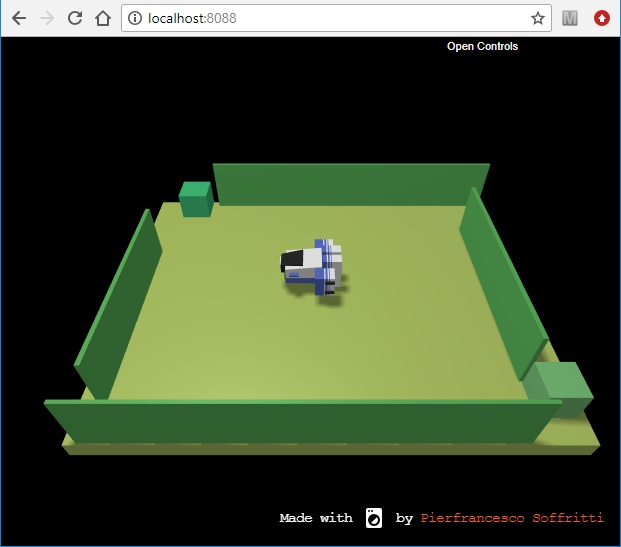
\includegraphics[scale=0.7]{img/virtualRobot.jpg}
	\caption{Esempio di pavimento con il robot in ambiente simulato}
	\label{fig:virtualrobot}
\end{figure}

Il robot lavora secondo le seguenti condizioni:
\begin{enumerate}
\item \code{R-Start}: un utente autorizzato (\code{authorized user}) ha inviato un comando \action{START} usando un'interfaccia \action{GUI} umana (\code{console}) in esecuzione su un normale \action{PC} oppure su uno smart device (\action{Android}).
\item \code{R-TempOk}: il valore di temperatura della città non è superiore ad un valore prefissato (per esempio 25\,$^{\circ}$ Celsius).
\item \code{R-TimeOk}: l'orario corrente è all'interno di un intervallo dato (per esempio fra le 7 e le 10 di mattina).
\end{enumerate}

Mentre il robot è in movimento:
\begin{itemize}
\item un \action{Led} posto su di esso deve lampeggiare, se il robot è un \fname{real} robot (\code{R-BlinkLed});
\item una \action{Led Hue Lamp} disponibile nella casa deve lampeggiare, se il robot è un \fname{virtual} robot (\code{R-BlinkHue});
\item deve evitare gli ostacoli fissi (per esempio i mobili) presenti nella stanza (\code{R-AvoidFix}) e/o gli ostacoli mobili come palloni, gatti, ecc. (\code{R-AvoidMobile}).
\end{itemize}

Inoltre il robot deve interrompere la sua attività quando si verifica una delle seguenti condizioni:
\begin{enumerate}
\item \code{R-Stop}: un utente autorizzato (\code{authorized user}) ha inviato il comando di \action{STOP} utilizzando la \code{console}.
\item \code{R-TempKo}: il valore di temperatura della città diventa più alto del valore prefissato.
\item \code{R-TimeKo}: l'orario corrente non è più all'interno dell'intervallo dato.
\item \code{R-Obstacle}: il robot ha trovato un ostacolo che non è in grado di evitare.
\item \code{R-End}: il robot ha finito il suo lavoro.
\end{enumerate}

Durante il suo funzionamento il robot può opzionalmente:
\begin{itemize}
\item \code{R-Map}: costruire una mappa del pavimento della stanza con la posizione degli ostacoli fissi. Una volta ottenuta, la mappa può essere utilizzata per definire un piano per un percorso (ottimo) dallo \code{start-point} all'\code{end-point}.
\end{itemize}

%=========================================================================

\section{Analisi dei requisiti}
\labelsec{ReqAnalysis}

I requisiti sono stati analizzati e formalizzati in modo iterativo in ordine di importanza, come riportato nel Product Backlog di Table \ref{tab:pb}. \\

% INSERISCI TABELLA PRODUCT BACKLOG
\begin{table}
	\centering
	\begin{tabular}{|l|c|}
		\hline \textbf{Requisito} & \textbf{Priorità} \\ \hline
		R-FloorClean & 1 \\ \hline
		R-Map & 2 \\ \hline
		R-AvoidFix & 3 \\ \hline
		R-AvoidMobile & 4 \\ \hline
		R-Obstacle & 5 \\ \hline
		R-BlinkHue & 6 \\ \hline
		R-BlinkLed & 6 \\ \hline
		R-Start & 7 \\ \hline
		R-TempOk & 7 \\ \hline
		R-TimeOk & 7 \\ \hline
		R-Stop & 7 \\ \hline
		R-TempKo & 7 \\ \hline
		R-TimeKo & 7 \\ \hline
		R-End & 7 \\ \hline
	\end{tabular} 
	\\[1\baselineskip]
	\caption{Product Backlog}
	\label{tab:pb}
\end{table}
Per formalizzare il requisito \code{R-FloorClean} è prima necessario stabilire cosa si intenda con pulire tutto il pavimento. Introducendo l'assunzione che la stanza sia rettangolare è possibile suddividerne la superficie in celle quadrate di dimensione fissa. Un modello della stanza è rappresentato in \ref{fig:grid}. 

\begin{figure}[h!]
	\centering
	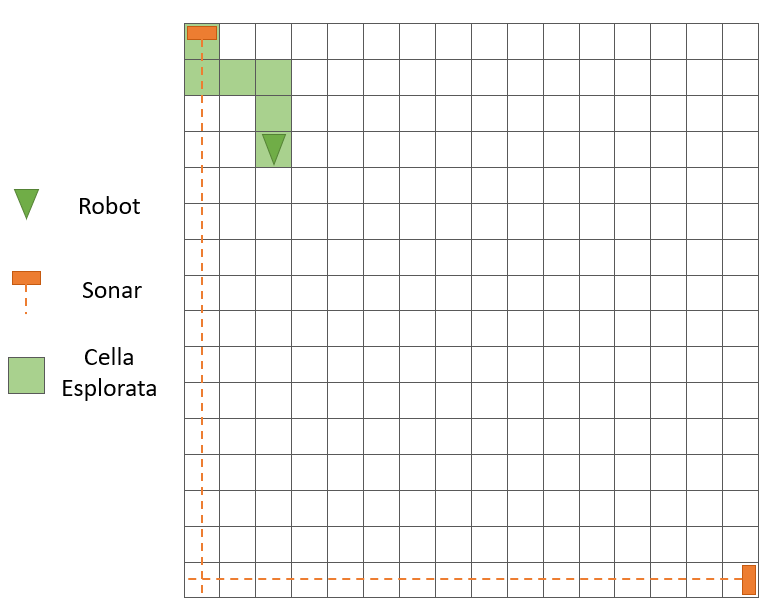
\includegraphics[scale=0.5]{img/grid.PNG}
	\caption{Modello a griglia della stanza}
	\label{fig:grid}
\end{figure}

Il lato delle celle dovrà essere di lunghezza non superiore al lato di dimensione maggiore del robot. Occorre quindi introdurre il concetto di \textbf{basic step}, ovvero un movimento che copra la distanza pari al lato della cella. Un basic step ha successo se il robot riesce ad avanzare nella cella successiva, mentre fallisce se la cella successiva è occupata da un ostacolo fisso. Al termine di un basic step la cella in cui il robot si trova è da considerarsi pulita. Qualsiasi percorso del robot dovrà essere espresso come una sequenza di basic step e di rotazioni di 90$^{\circ}$. \\ Fatte queste premesse, pulire tutta la stanza equivale a pulire ogni cella della stanza non occupata da un ostacolo fisso. Come da requisito \code{R-Map}, se è già stata costruita una mappa della stanza, il robot segue un percorso predefinito dallo \code{start-point} all'\code{end-point}, altrimenti procede nella pulizia della stanza costruendone la mappa. 

Il sistema da modellare è eterogeneo e distribuito, in particolare composto da almeno due nodi: il nodo "Robot" e il nodo "PC/Android". \\
Per la modellazione si utilizza il linguaggio \qa\ in quanto adatto alla modellazione di sistemi distribuiti. 

\begin{figure}[h]
	\centering
	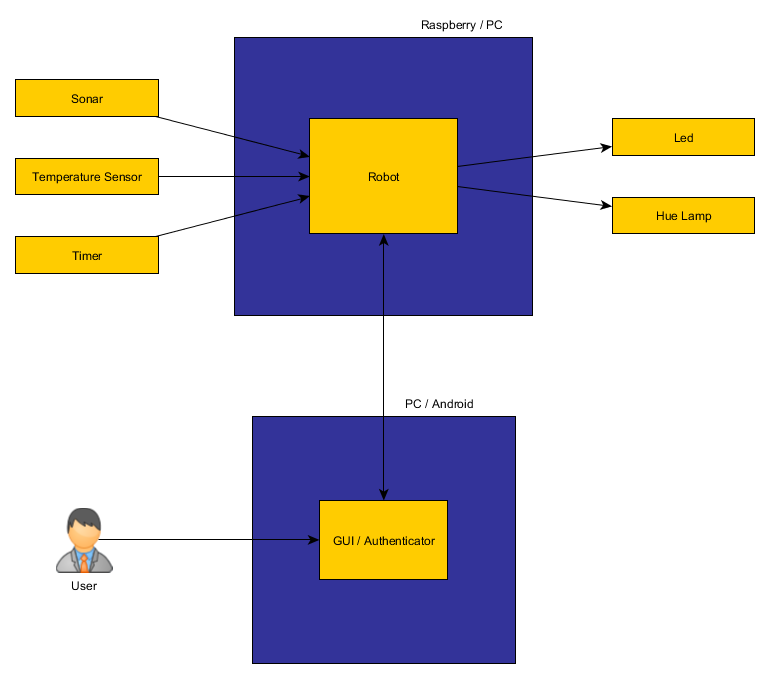
\includegraphics[scale=0.4]{img/requirements_analysis.png}
	\caption{Diagramma informale dell'analisi dei requisiti}
	\label{fig:reqAnalysis}
\end{figure}

Il primo dei due nodi ad essere modellato è il nodo "PC/Android" che si occupa di mostrare la \action{GUI} e di interagire direttamente con un utente umano, richiedendone l'autenticazione. Come da requisito \code{R-Start} l'interfaccia utente deve poter essere utilizzabile sia su \action{PC} che su un dispositivo \action{Android}. Tuttavia, essendo le funzioni che essa deve svolgere identiche in entrambi i casi, si sono rappresentati entrambi i nodi come un unico nodo. Su questo nodo esegue l'attore "GUI/Authenticator", che consente all'utente di autenticarsi e inviare i comandi di \action{START} e \action{STOP} al robot (\code{R-Start} e \code{R-Stop}). 

Il secondo nodo che si è modellato è il nodo "Raspberry/PC", responsabile del controllo del robot. Esso può essere in esecuzione su un PC, nel caso del \fname{virtual} robot, oppure su un Raspberry Pi nel caso del \fname{real} robot. \\ L'attore "Robot" si pone in attesa dei comandi inviati da "GUI/Authenticator" ed è in grado di ricevere informazioni relative alle condizioni di temperatura ed al tempo (\code{R-TempOk}, \code{R-TimeOk}, \code{R-TempKo}, \code{R-TimeKo}). Durante l'esecuzione, se il robot è in movimento, l'attore "Robot" invia a "Led" e a "Hue Lamp" i comandi per l'accensione e lo spegnimento necessari a farli lampeggiare (\code{R-BlinkLed}, \code{R-BlinkHue}). 

L'attore "Robot" si occupa inoltre di gestire la logica applicativa, che consiste, in seguito alla ricezione del comando \action{START} da parte dell'utente, nel prendere decisioni circa il movimento del robot all'interno della stanza – per il robot reale – e all'interno dell'ambiente simulato – per il robot virtuale – tentando di evitare gli ostacoli fissi e mobili (\code{R-AvoidFix}, \code{R-AvoidMobile}), costruendo una mappa del pavimento (\code{R-Map}) e interrompendone l'attività una volta completato il proprio lavoro (\code{R-End}).

Inoltre, se l'attore "Robot" trova un ostacolo che non riesce ad evitare si deve fermare (\code{R-Obstacle}).
Questa situazione si verifica quando il robot trova uno o più ostacoli che gli impediscono di raggiungere il secondo sonar.



Vengono di seguito riportati i modelli formali risultati dall'analisi dei requisiti che evidenziano una prima \textbf{architettura logica}:

\lstinputlisting[label={lst:reqAnalysisRobot}, title={\footnotesize reqAnalysisRobot.qa}]{../src/sprint\version/req_analysis/reqAnalysisRobot.qa}
\lstinputlisting[label={lst:reqAnalysisUser}, title={\footnotesize reqAnalysisUser.qa}]{../src/sprint\version/req_analysis/reqAnalysisUser.qa}

Trattandosi di un sistema eterogeneo distribuito, ed utilizzando il linguaggio di modellazione \action{QActor}, le due modalità con cui i componenti all'interno del sistema possono interagire sono quelle ad \textbf{eventi} e \textbf{messaggi}. 

In questo ambito un \textbf{messaggio} non è altro che un'informazione che il mittente invia ad uno \textbf{specifico destinatario}; al contrario, un \textbf{evento} cattura il concetto di informazione \textbf{senza specifico destinatario}: tutti i componenti del sistema interessati all'evento possono riceverlo. 

Dall'analisi dei requisiti sono emerse le necessità di interazione tra i sonar ed il robot, tra le sorgenti dei dati di temperatura e tempo ed il robot, nonché tra il robot stesso e i dispositivi attuatori, in questo caso led e lampada hue. \\
Sarebbe possibile modellare queste interazioni come messaggi: in questo caso sia i sonar che le sorgenti di temperatura e tempo dovrebbero conoscere lo specifico destinatario dei loro messaggi; allo stesso modo il robot dovrebbe conoscere i specifici dispositivi attuatori a cui inviare le informazioni. \\
Alla luce di ciò risulta più conveniente modellare queste interazioni tramite eventi, che permettono un maggiore disaccoppiamento delle entità in gioco, consentendo eventualmente a più robot distinti di raccogliere i dati in input e a differenti attuatori di ricevere comandi dal robot. 

Per quanto riguarda l'interazione user-GUI non si evidenziano particolari differenze nel modellarla tramite messaggi piuttosto che tramite eventi. 
Per quanto riguarda l'interazione gui-robot è più opportuno che essa sia modellata mediante eventi piuttosto che attraverso messaggi, in quanto risultano più vantaggiosi per disaccoppiare l'interfaccia grafica dallo specifico robot comandato. 

%=========================================================================

\section{Analisi del problema}
\labelsec{ProblemAnalysis}

Tenendo conto delle assunzioni e delle considerazioni già affrontate in analisi dei requisiti, il primo problema è posto dal requisito \code{R-FloorClean}. \\ Tale problema consiste nello stabilire una sequenza di movimenti che portino il robot a pulire il massimo numero di celle in cui è suddivisa la stanza. Nella stanza possono essere presenti degli ostacoli di varie forme e disallineati rispetto alla griglia. In quest'ultimo caso alcune celle potrebbero essere coperte solo parzialmente da degli ostacoli. Per semplicità, si considerano tali celle come totalmente coperte dagli ostacoli. Un esempio è riportato in figura \ref{fig:obstacles}.

\begin{figure}
	\centering
	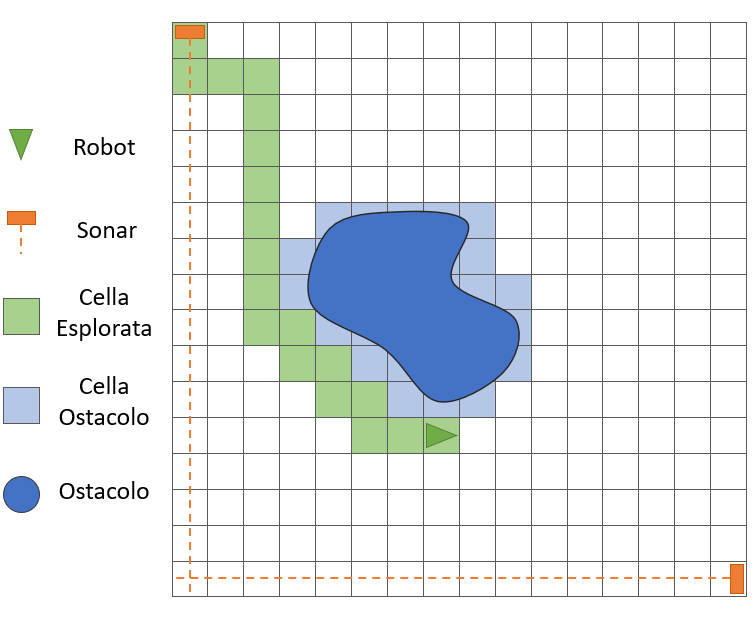
\includegraphics[scale=0.5]{img/obstacle.PNG}
	\caption{Esempio di ostacolo fisso nella stanza}
	\label{fig:obstacles}
\end{figure}

Gli ostacoli presenti nella stanza possono essere classificati in fissi e mobili:
\begin{itemize}
	\setlength\itemsep{0em}
	\item gli ostacoli fissi occupano le stesse celle per una durata indefinita;
	\item gli ostacoli mobili si spostano dalla cella precedentemente occupata in un'altra cella allo scadere di un dato intervallo di tempo.
\end{itemize}
Il robot deve essere in grado di pulire le celle momentaneamente occupate da ostacoli mobili. \\
Nel caso in cui vi siano celle non occupate ma irraggiungibili, tali celle vengono considerate come ostacoli fissi.

Per pulire la stanza in autonomia, il robot ha accesso a tre tipi di informazione:
\begin{itemize}
	\setlength\itemsep{0em}
	\item la prima è fornita dal sonar montato sulla parte anteriore del robot, in grado di rilevare un ostacolo immediatamente davanti al robot;
	\item la seconda riguarda invece le distanze dal \code{sonar1} e dal \code{sonar2}, posizionati come in figura \ref{fig:virtualrobot};
	\item la terza riguarda i dati memorizzati durante l'esplorazione della stanza (ad esempio la mappa della stanza).
\end{itemize}
Per semplicità, si assume che non ci siano ostacoli nel raggio di azione dei due sonar presenti nella stanza. \\
L'unico modo che ha il robot per rilevare la presenza di un ostacolo è tentare di effettuare un basic step nella direzione desiderata e mettersi in ascolto dell'evento emesso dal sonar anteriore.

\begin{comment}
Il requisito \code{R-FloorClean} è stato modellato attraverso l'introduzione del QActor \textbf{robotmind}. \\ Quest'ultimo possiede una propria base di conoscenza necessaria a tenere traccia delle dimensioni della stanza e della direzione corrente del robot. Tale QActor è sensibile ai messaggi \textbf{robotMindCmd} ed agli eventi \textbf{sensorEvent}, in particolare:
\begin{itemize}
	\item alla ricezione del messaggio \textbf{robotMindCmd : robotMindCmd(explore)} viene invocato il metodo statico \textbf{doBasicStep()} della classe Java \textbf{robot}, a cui viene delegata l'esecuzione del basic step del robot. Questo metodo deve tenere conto degli eventi \textbf{sensorEvent : sensorEvent(onboardsonar)} per determinare quando il robot si è imbattuto in un ostacolo, che secondo le precedenti assunzioni viene a coincidere con il secondo sonar. In seguito a ciò viene discriminato il buon esito del basic step, determinato dalla presenza o dall'assenza di un ostacolo lungo il percorso del robot. A seconda della direzione del robot vengono incrementate le dimensioni della stanza. Il caso di fallimento del basic step in questa fase di cosiddetta "esplorazione" si verifica quando il robot colpisce il secondo sonar: in tal caso vengono invocati i metodi statici della classe \textbf{planner} necessari ad indicare al planner le dimensioni della stanza per poi passare alla fase di pulizia della stanza vera e propria con l'invio del messaggio \textbf{robotMindCmd : robotMindCmd(clean)}.
	\item alla ricezione dell'evento \textbf{sensorEvent : sensorEvent(sonar2)} viene modificata la direzione del robot memorizzata nella base di conoscenza;
	\item alla ricezione del messaggio \textbf{robotMindCmd : robotMindCmd(clean)} viene dapprima invocato il metodo statico \textbf{nextMove()} della classe Java \textbf{planner}, dove per planner si intende un'entità a conoscenza delle dimensioni della stanza in grado di determinare la prossima mossa del robot (basic step o basic step + rotazione di 90 gradi), inserita nella base di conoscenza di volta in volta, col fine di coprire l'intera area della stanza. A seconda della mossa indicata dal planner vengono invocati i metodi statici della classe \textbf{robot} necessari ad eseguire la mossa. \\ La pulizia della stanza si intende conclusa quando viene aggiunto dal planner alla base di conoscenza il fatto \textbf{nextMove(n,n)}, che indica al robot di non eseguire nessun movimento ulteriore. 
\end{itemize}
\end{comment}

Per poter entrare in esecuzione, il robot deve ricevere un comando \action{START} da un utente autorizzato. Sorge dunque il problema di stabilire quale tra i due nodi, riportati in figura \ref{fig:reqAnalysis}, si occuperà di autenticare l'utente. \\ Una possibilità è quella di relegare l'autenticazione al nodo del robot: in questo caso il robot potrebbe non disporre delle adeguate risorse computazionali per gestire il processo di autenticazione, tuttavia questo garantirebbe maggiore sicurezza. \\ Un'altra possibilità è che l'autenticazione venga gestita da un nodo diverso rispetto a quello del robot: ciò consentirebbe di non utilizzare le risorse computazionali del robot richiedendo però maggiori accortezze sulla sicurezza. In quest'ultimo caso l'autenticazione potrebbe essere gestita dal nodo dell'utente oppure da un nodo distinto, il quale comporterebbe costi maggiori. \\

Un altro problema è quello relativo all'interfaccia \action{GUI} che l'utente utilizza per interagire con il robot. Questa interfaccia deve poter eseguire su dispositivi eterogenei. A tal proposito, una possibilità sarebbe creare client nativi per ogni piattaforma con costi elevati oppure più semplicemente utilizzare una pagina web. 

La comunicazione tra utente e robot tramite \action{GUI} può avvenire via messaggi o via eventi. La comunicazione ad eventi permette di disaccoppiare \action{GUI} e robot, consentendo di utilizzare un'unica \action{GUI} per comunicare con diversi robot. Utilizzando gli eventi può essere adottato un approccio \code{event-based} o un approccio \code{event-driven}. Nell'approccio \code{event-based} il robot non sarebbe sempre sensibile agli eventi, potendone perdere alcuni. Al contrario, nell'approccio \code{event-driven} il robot sarebbe sempre sensibile agli eventi perdendo tuttavia reattività.

% INSERIRE ANALISI BLINKING
% INSERIRE ANALISI TEMPOK E TIMEOK
% INSERIRE DISCUSSIONE SPRINT E APPROCCIO INCREMENTALE-EVOLUTIVO (REQUISITI NON CONSIDERATI TUTTI INSIEME) 

Vengono di seguito riportati i modelli formali prodotti dall'analisi del problema, in cui viene delineata l'\textbf{architettura logica} del sistema risultante dalla fase di analisi: 

\lstinputlisting[label={lst:probAnalysisRobot},title={\footnotesize probAnalysisRobot.qa}]{../src/sprint5/prob_analysis/probAnalysisRobot.qa}
\lstinputlisting[label={lst:probAnalysisUser},title={\footnotesize probAnalysisUser.qa}]{../src/sprint5/prob_analysis/probAnalysisUser.qa}

%=========================================================================

\section{Progettazione}
\labelsec{Project}
%=========================================================================

\begin{comment}
\lstinputlisting[label={lst:designResourseModel},title={\footnotesize resourceModel.qa}]{../src/sprint\version/impl/it.unibo.finaltask2018.impl/src/resourceModel.qa}
\lstinputlisting[label={lst:designOut},title={\footnotesize output.qa}]{../src/sprint\version/impl/it.unibo.finaltask2018.impl/src/output.qa}
\lstinputlisting[label={lst:designIn}, title={\footnotesize input.qa}]{../src/sprint\version/impl/it.unibo.finaltask2018.impl/src/input.qa}
\lstinputlisting[label={lst:designAppl},title={\footnotesize applicationLogic.qa}]{../src/sprint\version/impl/it.unibo.finaltask2018.impl/src/applicationLogic.qa}
\lstinputlisting[label={lst:designIn}, title={\footnotesize real\_robot\_adapter.qa}]{../src/sprint\version/design/it.unibo.finaltask2018.design/src/real_robot_adapter.qa}
\lstinputlisting[label={lst:designIn}, title={\footnotesize real\_led\_adapter.qa}]{../src/sprint\version/design/it.unibo.finaltask2018.design/src/real_led_adapter.qa}
\end{comment}


\section{Implementazione}
\labelsec{Implementation}
%===========================================================================
% INSERIRE COMMENTO SU MYPLANNER: INTERFACCIA CON IL PIANIFICATORE MESSO A DISPOSIZIONE
\lstinputlisting[label={lst:designResourseModel},title={\footnotesize resourceModel.qa}]{../src/sprint\version/impl/it.unibo.finaltask2018.impl/src/it/unibo/myPlannerIntegrator/myPlanner.java}
% INSERIRE FILES FRONTEND SERVER E RELATIVI COMMENTI
L'implementazione del frontend server, necessario per fornire all'utente la possibilità di autenticarsi e quindi di dare i comandi di inizio e stop al robot, è avvenuta in \node, sfruttando il framework Express. In figura \ref{fig:frontend} è presente un modello informale che rappresenta le tecnologie utilizzate nell'integrazione fra il frontend server e l'infrastruttura \qa\ già presente.

\begin{figure}
	\centering
	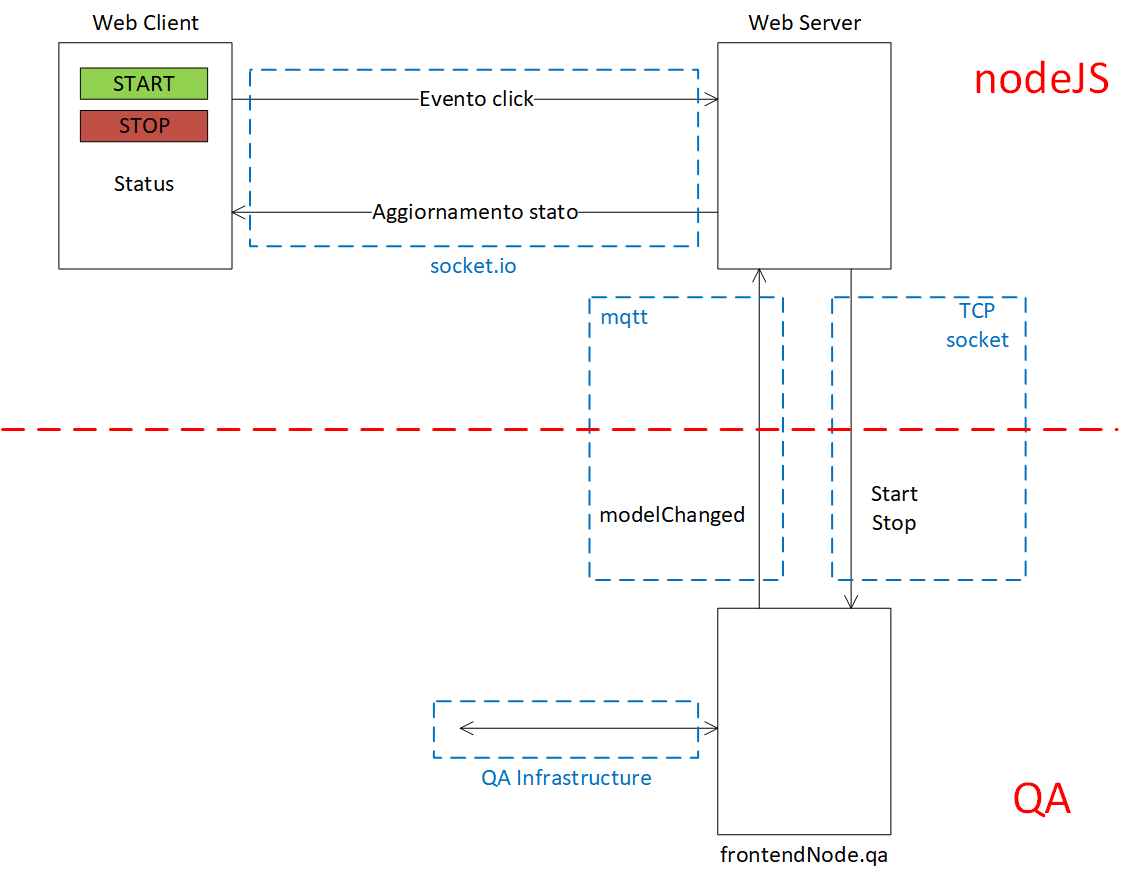
\includegraphics[scale=0.5]{img/frontend.png}
	\caption{Architettura informale che rappresenta l'integrazione del frontend server con l'infrastruttura \qa}
	\label{fig:frontend}
\end{figure}

Come si può vedere la comunicazione tra la pagina web fornita all'utente e il server web avviene tramite \action{socket.io} e rimane pienamente in ambiente \node. La comunicazione con l'infrastruttura \qa\ utilizza invece una \action{TCP socket} nativa del contesto; la comunicazione nella direzione opposta avviene invece tramite un server \action{mqtt}.

%===========================================================================
%\section{Testing}
%\labelsec{Testing}
%===========================================================================
%
%===========================================================================
%\section{Maintenance}
%\labelsec{Maintenance}
%===========================================================================
%
%===========================================================================
%\section{Deployment}
%\labelsec{Deployment}
%
%===========================================================================
\newpage
%\section{Authors}
\section{Autori}
\labelsec{Authors}
%===========================================================================

\vskip.5cm
%
% I nostri nomi sono authA, authB, authC in ordine alfabetico.
%
\begin{table}
\begin{tabular}{|c|c|c|}
\hline
\multicolumn{3}{|c|}{Foto degli autori} 
\\
\hline
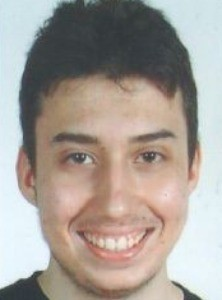
\includegraphics[scale = 0.4]{img/foto_authA.jpg}&
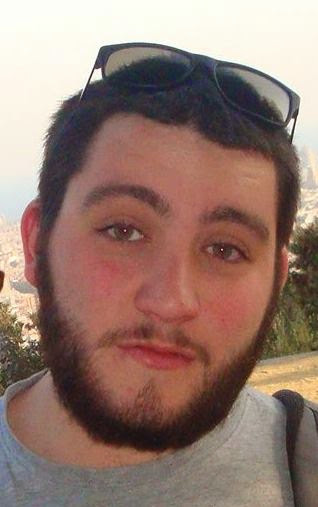
\includegraphics[scale = 0.26]{img/foto_authB.jpg}&
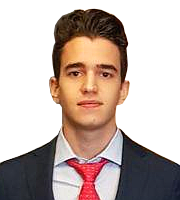
\includegraphics[scale = 1.0]{img/foto_authC.png}
\\
\hline
\xauthA& \xauthB& \xauthC
\\
\hline
\end{tabular}
\end{table}



\end{document}












